In this section we demo some of the interactive designs elements which we
believe will be be important in realizing our vision for the final product.

\subsection{Command Info}

\begin{figure}[H]
  \centering
  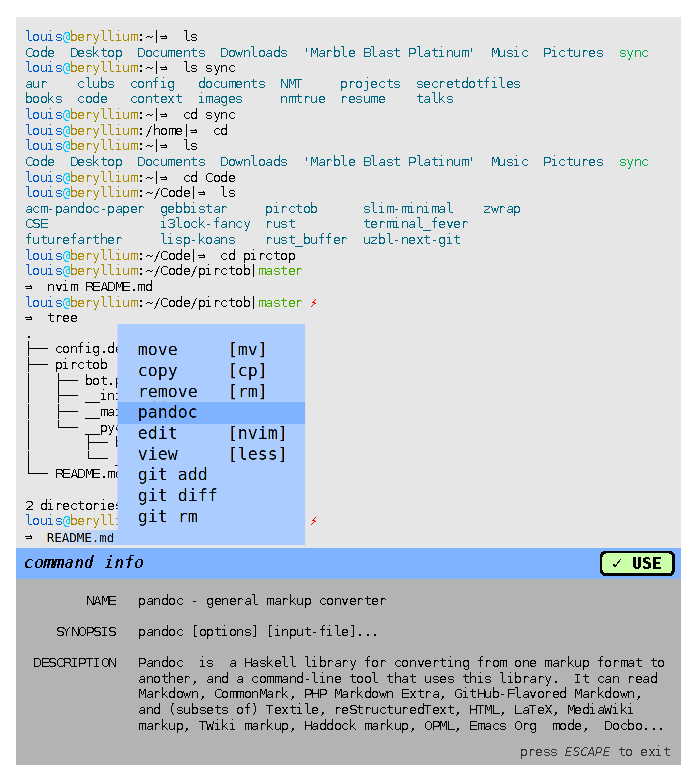
\includegraphics[width=0.8\linewidth]{figures/interface/files.eps}
  \caption{A mockup of the autocomplete dialog with the command info window}
  \label{fig:cmdinfo}
\end{figure}

Figure \ref{fig:cmdinfo} illustrates our idea for the autocomplete dialog. The
user can access the dialog by tab-completing the command they are typing, or
clicking on a the name of a file in the output of any command. The dialog box
can show a list of possible commands, determining which suggestions are most
likely based on command history, the current working context, or the type of the
file to be acted on. The autocomplete open remains open, leaving the user a
trail of ``breadcrumbs'' which can lead them back to other commands' information
windows.

The command info window is parsed from the man pages of the suggested commands,
and the layout is right/left aligned to make it easier to read. The window is
mainly a menu page for the particular command the user is interested in, but
doubles as an input form for the CLI. The possible command line options that
will appear in the documentation can be treated as form controls, (conceptually
similar to checkboxes), which allow the user to interactively build commands by
clicking or tabbing through.

\subsection{Automation Helper}

\begin{figure}[H]
  \centering
  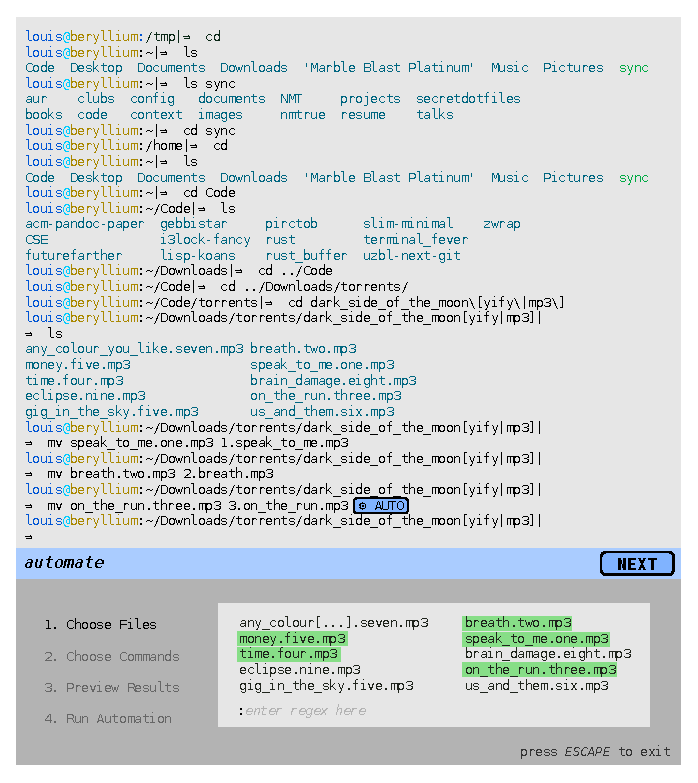
\includegraphics[width=0.8\linewidth]{figures/interface/automation.eps}
  \caption{An example use of the automation window}
  \label{fig:autow}
\end{figure}

One of the main things that makes the command line powerful, and one of the
hardest features to use effectively, is the ability to automate common system
tasks. Figure \ref{fig:autow} shows an example interface for a feature which can
guide users through the process of automating tasks. The interface makes use of
the users command history to detect when the same command has been used several
times in the row, and presents the user with a button to bring up the automation
window \--- this follows from the concept of responsive enabling.

The automation window is a sequence map that walks the user through the steps of
creating a loop in their shell's language to repeat a task multiple times. In
this example, the terminal is helping the user iterate over file names, so it
creates a form where the user can select files, (again, similar to checkboxes),
to add to the loop. There is also a textbox where the user can input formatted
text to select files with shell wildcards \--- this is indicated to the user by
adding an input hint to the form.

\subsection{Undo Window}

\begin{figure}[H]
  \centering
  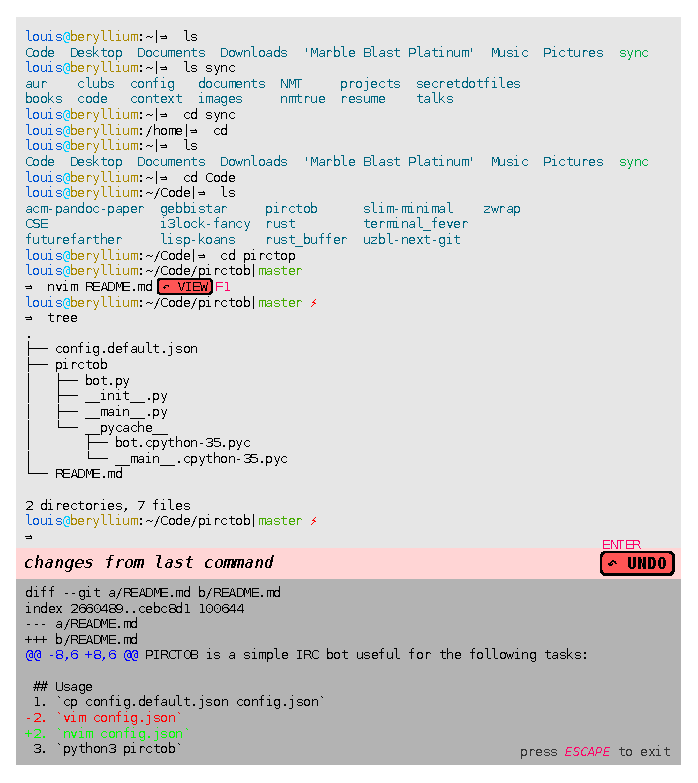
\includegraphics[width=0.8\linewidth]{figures/interface/undo.eps}
  \caption{A mockup of the undo window with undo option}
  \label{fig:undo}
\end{figure}

In Figure \ref{fig:undo} we can see an example interface for the undo window for
our terminal. After a command is entered that changes something, this shows the
user exactly what changes have taken place, and makes it possible to undo the
last set of changes. After any state-altering command is entered at the CLI, a
button is appended to the command in the log which brings up the shown
dialog. The same dialog can be made available from the heads-up display in the
bottom, or the terminal can be configured to show the undo window after
destructive commands by default.

The point of this interface is to create an escape hatch to allow the user to
return the entire system to the state before the previous command. This is an
example of responsive disclosure, because the information is only made available
to the user when they indicate that they want to know how to undo a command. The
system is also inherently limited in that it can only undo a single command, so
as more commands are entered the button should disappear from older commands
that can no longer be undone. This follows the principle of responsive enabling.

The undo button closes the pane by undoing the command, and pressing
\texttt{ESC} simply returns the user to the normal context window without
undoing anything. Both are examples of having a prominent ``done'' button, so
the user knows how to tell the terminal they're done with the undo dialog. The
red color on the dialog window also serves as a visual warning to the user to
indicate that what they are doing will ultimately result in a real change to the
state of the system, to make them more likely to exercise proper caution.
